\newpage

\section{Partitionierung}

\subsubsection{Grundlagen}

\begin{itemize}
  \item ungerichtete Distanzadjazenzmatrix $\gls{Adist} \in \gls{R+}^{N \times N} = {\left(a\right)}_{ij}$
  \item (lokal) normalisierte ungerichtete Distanzadjazenzmatrix $\gls{Adistnorm} \in \gls{R+}^{N \times N} = {\left(\tilde a\right)}_{ij}$
  \item gerichtete Winkeladjazenzmatrix $\gls{Arad} \in \gls{R+}^{N \times N} = {\left(\alpha\right)}_{ij}$
  \item Input-Featurematrix $\gls{F} \in \gls{R}^{N \times X} = {\left(f\right)}_{ij}$
  \item Output-Featurematrix $\gls{Fout} \in \gls{R}^{N \times Y} = {\left(f^{\prime}\right)}_{ij}$
  \item Anzahl Partitionen $P$
  \item Gewichtstensor $\ma{W} \in \gls{R}^{\left(P + 1\right) \times X \times Y} = {\left(w\right)}_{ijw}$
\end{itemize}

\subsubsection{Faltung}

\begin{equation}
  f^{\prime}_{iy} = \sum_{x = 1}^X f_{ix} \cdot w_{\left(P +1\right)xy} \sum_{n = 1}^N \tilde a_{in} \cdot f_{nx} \cdot b^K_P\left(\alpha_{in}, x, y\right)
\end{equation}
wobei $b_P^K$ eine B-Spline-Kurve.

Es ist anzumerken, dass \gls{Adistnorm} keine Schleifen enthalten sollte, da für diese kein Wert in der Winkelmatrix Sinn macht.
Deswegen wird der zu betrachtende Knoten in der Faltung jeweils einzeln mit einem Gewicht multipliziert.

\todo{Matrixschreibweise}

\subsubsection{B-Spline-Kurven}

$b_P^K \colon \left]0, 2\pi\right] \times \left\{1, \ldots, X \right\} \times \left\{1, \ldots, Y\right\} \to \gls{R}$ ist eine B-Spline-Kurve der Ordnung $K \in \gls{N}$ auf den Kantenwinkeln des Graphen.
Bemerke, dass wir $0$ für Winkel aussschließen und stattdessen den Winkel $2\pi$ benutzen, so dass wir nicht mit der Bedeutung von $0$ bei Adjazenzmatrizen in die Quere kommen.
\begin{equation}
  b_P^K\left(\alpha, x, y \right) = \sum_{p=1}^P w_{pxy} \cdot e_p^K\left(\alpha\right)
\end{equation}
wobei die Basisfunktion $e_p^K$ rekursiv über $K$ definiert ist mit Initialisierung
\begin{equation}
  e_p^0\left(\alpha\right) = \begin{cases}
    1, & \text{wenn }s\left(p-1\right) < \alpha \leq s\left(p\right)\text{,}\\
    0, & \text{sonst}
  \end{cases}
\end{equation}
und Rekursionsschritt
\begin{equation}
  e_p^k\left(\alpha\right) = \frac{\alpha - s\left(p-1\right)}{s\left(p\right) - s\left(p-1\right)} e_{p-1}^{k-1}\left(\alpha\right) + \frac{s\left(p+1\right) - \alpha}{s\left(p+1\right) - s\left(p\right)} e_p^{k-1}\left(\alpha\right)
\end{equation}
wobei $s \colon \gls{N} \to \left]0, 2\pi\right]$ mit
\begin{equation}
  s\left(p\right) = \begin{cases}
    \frac{2p\pi}{P} & \text{wenn }1 \leq p \leq P\text{,}\\
    s\left(1\right) & \text{wenn }p > P\text{,}\\
    s\left(P\right) & \text{sonst.}
  \end{cases}
\end{equation}
Es ist anzumerken, dass wir $s$ dabei für den Rekursionsschritt über die Grenzen $1$ und $P$ hinaus definieren.
Das hilft uns, die B-Spline-Kurve \emph{kreisförmig} abzuschließen.

Je größer $K$ gesetzt wird, umso mehr Anteile anderer benachbarter Stützpunkte fließen in die Berechnung mit ein.
Die Größe von $K$ wird deshalb auch oft \emph{lokale Kontrollierbarkeit} genannt.

\subsubsection{Beispiel mit $P=4$}

\begin{center}
\begin{tikzpicture}
  \begin{axis}[xmax=4.5,
               xmin=0,
               ymin=0,
               ymax=1.25,
               xlabel={$\alpha$},
               ylabel={$e_p^1$},
               xtick={1, 2, 3, 4},
               xticklabels={$\frac{\pi}{2}$, $\pi$, $\frac{3\pi}{2}$, $2\pi$},
               ytick={1},
               axis equal,
               axis x line=center,
               axis y line=center,
               xlabel style={below right},
               ylabel style={above left},
               legend pos=outer north east]
    \addplot [ultra thick, brown] coordinates {(0,1)(1,1)};
    \addlegendentry{$p = 1$}
    \addplot [ultra thick, blue] coordinates {(1,1)(2,1)};
    \addlegendentry{$p = 2$}
    \addplot [ultra thick, red] coordinates {(2,1)(3,1)};
    \addlegendentry{$p = 3$}
    \addplot [ultra thick, green] coordinates {(3,1)(4,1)};
    \addlegendentry{$p = 4$}
  \end{axis}
\end{tikzpicture}
\end{center}

\begin{center}
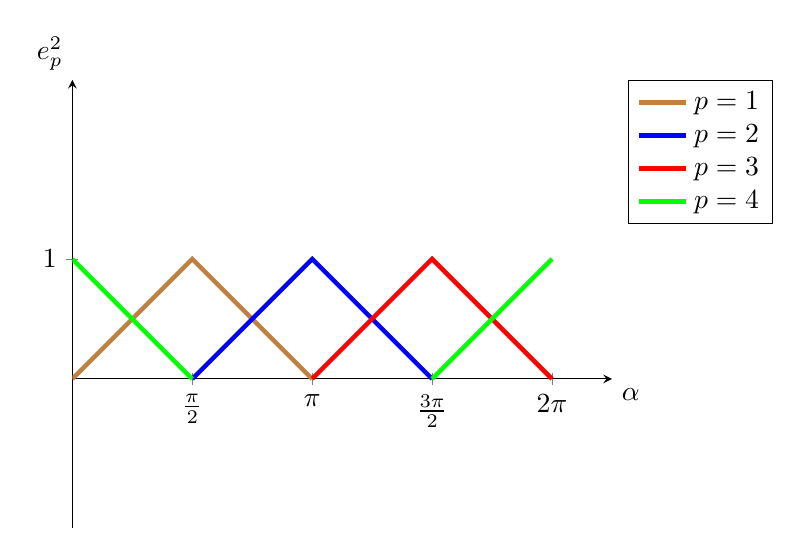
\begin{tikzpicture}
  \begin{axis}[xmax=4.5,
               xmin=0,
               ymin=0,
               ymax=1.25,
               xlabel={$\alpha$},
               ylabel={$e_p^2$},
               xtick={1, 2, 3, 4},
               xticklabels={$\frac{\pi}{2}$, $\pi$, $\frac{3\pi}{2}$, $2\pi$},
               ytick={1},
               axis equal,
               axis x line=center,
               axis y line=center,
               xlabel style={below right},
               ylabel style={above left},
               legend pos=outer north east]
    \addplot [ultra thick, brown] coordinates {(0,0)(1,1)(2,0)};
    \addlegendentry{$p = 1$}
    \addplot [ultra thick, blue] coordinates {(1,0)(2,1)(3,0)};
    \addlegendentry{$p = 2$}
    \addplot [ultra thick, red] coordinates {(2,0)(3,1)(4,0)};
    \addlegendentry{$p = 3$}
    \addplot [ultra thick, green] coordinates {(3,0)(4,1)};
    \addlegendentry{$p = 4$}
    \addplot [ultra thick, green] coordinates {(0,1)(1,0)};
  \end{axis}
\end{tikzpicture}
\end{center}


\subsection{Anwendung auf Faltungsebene}



\subsection{Konstante Partitionierung}

\subsection{Lineare Partitionierung}

% Das ganze lässt sich eleganter als Matrixmultiplikation schreiben:
% \begin{equation}
%   \gls{Fout} = \gls{Adistnorm} \cdot \gls{F} \cdot p_P^K\left(\gls{Arad}\right)
% \end{equation}
% \todo{das stimmt nicht, was returned $p$ bei Matrizen}

% \begin{itemize}
%   \item Graphen konstant partitionieren (zum Beispiel in 8 Bereiche) $\rightarrow$ Graph ist nun gerichtet
%   \item Graphen linear partitionieren (Jans Idee)
% \end{itemize}

% \todo{Stichwort B-Spline}
% Angenommen wir haben $n=4$ Partitionierungen, dann haben wir $4$ Gewichte.
% Wir wollen die ganze Scheiße nicht einzeln partitionieren, sondern die Adjazenzmatrix einfach so betrachten.

% Dazu wird eine Funktion $f \colon \left[ 0, 2\pi \right] \to \left[ 0, 1 \right]$ approximiert bzw.\ gelernt.
% Sie besteht aus $n + 1$ Stützstellen $s$, wobei $s_0 = s_n$.
% Diese Stützstellen fungieren wie die Basisfunktion der B-Splines erster Ordnung.
% Sie formen lineare Hüte $N_i\left(x\right)$ bis zu ihren Nachbarstützstellen und sind im restlichen Teilintervallen $0$.
% Die $y$-Koordinate der Stützstellen sind die Gewichte.
% Die Stützstellen sind homogen im Intervall verteilt.

% Dann ist $f$ wie folgt definiert:

% \begin{equation*}
%   f\left(x\right) = \sum_{i=0}^n s_i \cdot N_i^n\left(x\right)
% \end{equation*}

% wobei

% \begin{equation*}
%   N_i^n\left(x\right) = \min \left( \max \left( E_i^n\left( x \right), 0 \right) 1 \right)
% \end{equation*}

% und

% \todo{basisfunktion angucken}

% \begin{equation}
%   E_i^n\left(x \right) =
% \end{equation}

% Teilbereiche haben die Größe $\frac{2\pi}{n}$.

% Ok, jetz habe ich das.
% Das heißt ich kann jetz für eine Kante dessen Gewichtsmultiplikation bestimmen.

% Wie war das nochmal.
% Ich habe $A$ und $F$ und $W$.


% $\gls{A}_{\text{rad}}$ ist $N \times N$, $\ma{F}$ ist $N \times X$ und $W$ ist $P \times X \times Y$ und da soll rauskommen $F'$ ist $N \times Y$.
% Ich habe $p$ Partitionen.

% Dann berechnet sich die Convolution für ein Feld wie folgt:

% Jetz muss ich $A_{\text{rad}}$ umwandeln, d.h.\ elementweise Multiplikation mit $f$.
